\documentclass{beamer}

\usepackage{graphicx}
\usepackage{booktabs}
\usepackage{hyperref}

\title{CartPole RL Enhancement}
\subtitle{A Deep Reinforcement Learning Approach with Curriculum Learning and Energy Consumption Optimization}
\author{Louis Gauthier}
% \institute{Your Institution}
\date{\today}

\begin{document}

\frame{\titlepage}

\begin{frame}
\frametitle{Table of Contents}
\tableofcontents
\end{frame}

\section{Project Overview}

\begin{frame}
\frametitle{Project Overview}
\begin{itemize}
    \item \textbf{Objective:} Enhance the classic CartPole environment by introducing a third action ("Do Nothing") and develop a deep RL solution to manage the modified environment.
    \item \textbf{Key Features:}
    \begin{itemize}
        \item Addition of a neutral action to the action space.
        \item Implementation of curriculum learning to adjust reward weights dynamically.
        \item Incorporation of temperature-scaled softmax for exploration-exploitation balance.
        \item Logging and monitoring using TensorBoard.
        \item Energy consumption as a reward component.
    \end{itemize}
    \item \textbf{Outcome:} Achieved a high success rate with efficient energy usage after 100k training steps.
\end{itemize}
\end{frame}

\section{Environment Description}

\begin{frame}
\frametitle{Environment Description}
\begin{itemize}
    \item \textbf{Classic CartPole:}
    \begin{itemize}
        \item Two actions: Apply a force to the cart to push it left or right.
        \item Observation Space: Cart position, cart velocity, pole angle, pole angular velocity.
        \item Objective: Balance the pole by moving the cart. Episode ends if pole angle exceeds a threshold or cart moves out of bounds.
    \end{itemize}
\end{itemize}

% TODO: Insert a diagram illustrating the classic vs. modified CartPole environments.
% Example Image: Compare classic CartPole with the modified version showing the additional "Do Nothing" action.
\begin{figure}[ht]
    \centering
    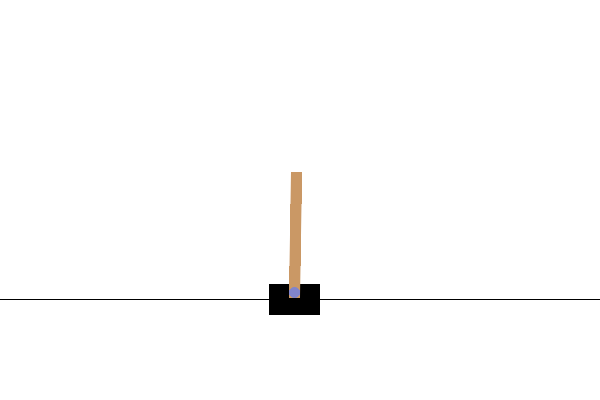
\includegraphics[width=0.7\textwidth]{images/cart_pole.png}
    \caption{The CartPole Environments}
    \label{fig:env_comparison}
\end{figure}
\end{frame}

\begin{frame}
\frametitle{Environment Description}
\begin{itemize}
    \item \textbf{Modified CartPole:}
    \begin{itemize}
        \item \textbf{Third Action:} \textit{Do Nothing} - No force applied to the cart.
        \item \textbf{Reward Structure:} Split into four equal components: Alive, Distance to Center, Pole Angle, and Energy Usage.
        \item \textbf{Curriculum Learning:} Adjusts reward weights based on training phases.
    \end{itemize}
\end{itemize}

\begin{figure}[ht]
    \centering
    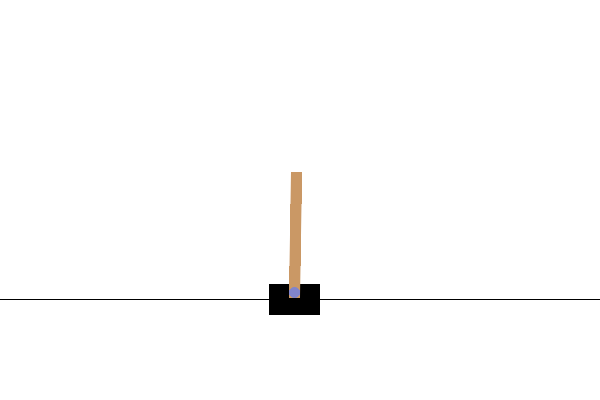
\includegraphics[width=0.7\textwidth]{images/cart_pole.png}
    \caption{The CartPole Environments}
    \label{fig:env_comparison}
\end{figure}
\end{frame}

\section{Steps Towards the Solution}

\begin{frame}
\frametitle{Steps Towards the Solution}
\begin{enumerate}
    \item \textbf{Environment Modification:}
    \begin{itemize}
        \item Added a third "Do Nothing" action to the action space.
        \item Adjusted the reward function to incorporate energy consumption.
    \end{itemize}
    \item \textbf{Algorithm Development:}
    \begin{itemize}
        \item Implemented a combination of Double DQN and Dueling DQN for stable learning.
        \item Used a target network to improve training stability.
        \item Utilized Prioritized Experience Replay to sample important transitions.
        \item Applied Gradient Clipping to prevent exploding gradients.
    \end{itemize}
    \item \textbf{Enhancements:}
    \begin{itemize}
        \item Introduced Curriculum Learning to adjust reward weights dynamically.
        \item Integrated Temperature-Scaled Softmax for exploration-exploitation balance.
        \item Tested Normalization for observations and rewards.
    \end{itemize}
\end{enumerate}
\end{frame}

\begin{frame}
\frametitle{Steps Towards the Solution}
\begin{figure}[ht]
    \centering
    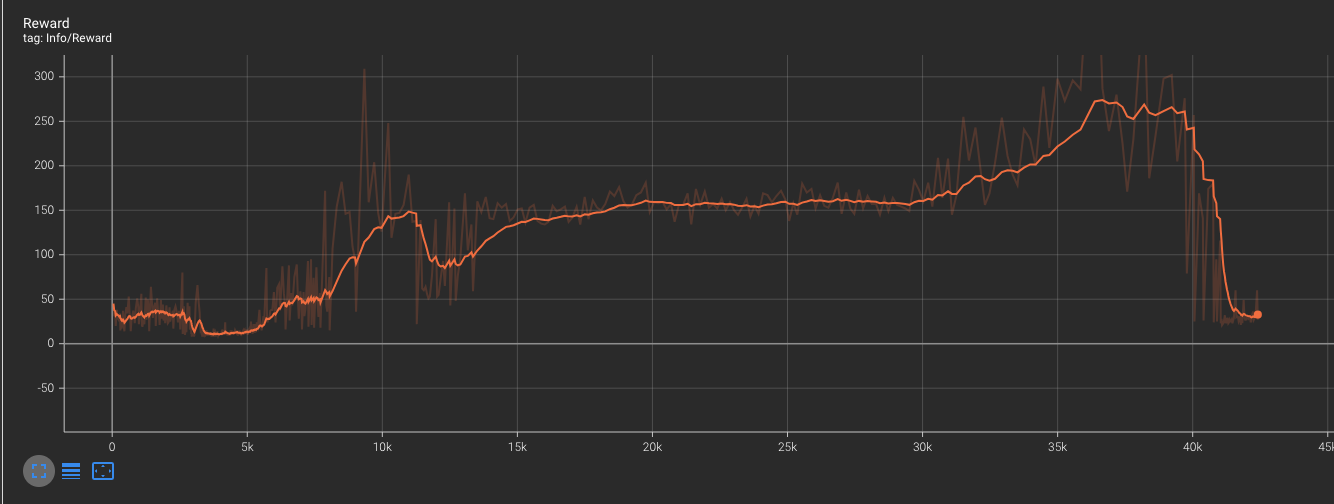
\includegraphics[width=1.0\textwidth]{images/catastrophic_forgetting.png}
    \caption{Catastrophic Forgetting occuring in the training process}
    \label{fig:catastrophic_forgetting}
\end{figure}
\end{frame}

\begin{frame}
\frametitle{Steps Towards the Solution}
\begin{enumerate}
    \setcounter{enumi}{3}
    \item \textbf{Problems encountered:}
    \begin{itemize}
        \item Catastrophic forgetting: The agent forgets previously learned behaviors.
        \begin{itemize}
            \item Solution: Use non-deterministic actions and temperature scheduling.
        \end{itemize}
        \item Reward function is not a good metric of performance during training.
        \begin{itemize}
            \item Solution: Run evaluations every 2k steps to track performance.
        \end{itemize}
    \end{itemize}
    \item \textbf{Logging and Monitoring:}
    \begin{itemize}
        \item Set up TensorBoard for real-time monitoring of training metrics.
        \item Logged individual sub-rewards and penalties for detailed analysis.
        \item Evaluation every 2k steps to track performance.
    \end{itemize}
    \item \textbf{Checkpointing:}
    \begin{itemize}
        \item Enabled resuming training from saved checkpoints.
        \item Handling crashes or interruptions during training.
    \end{itemize}
\end{enumerate}
\end{frame}

\begin{frame}
\frametitle{TensorBoard Metrics}
\begin{figure}[ht]
    \centering
    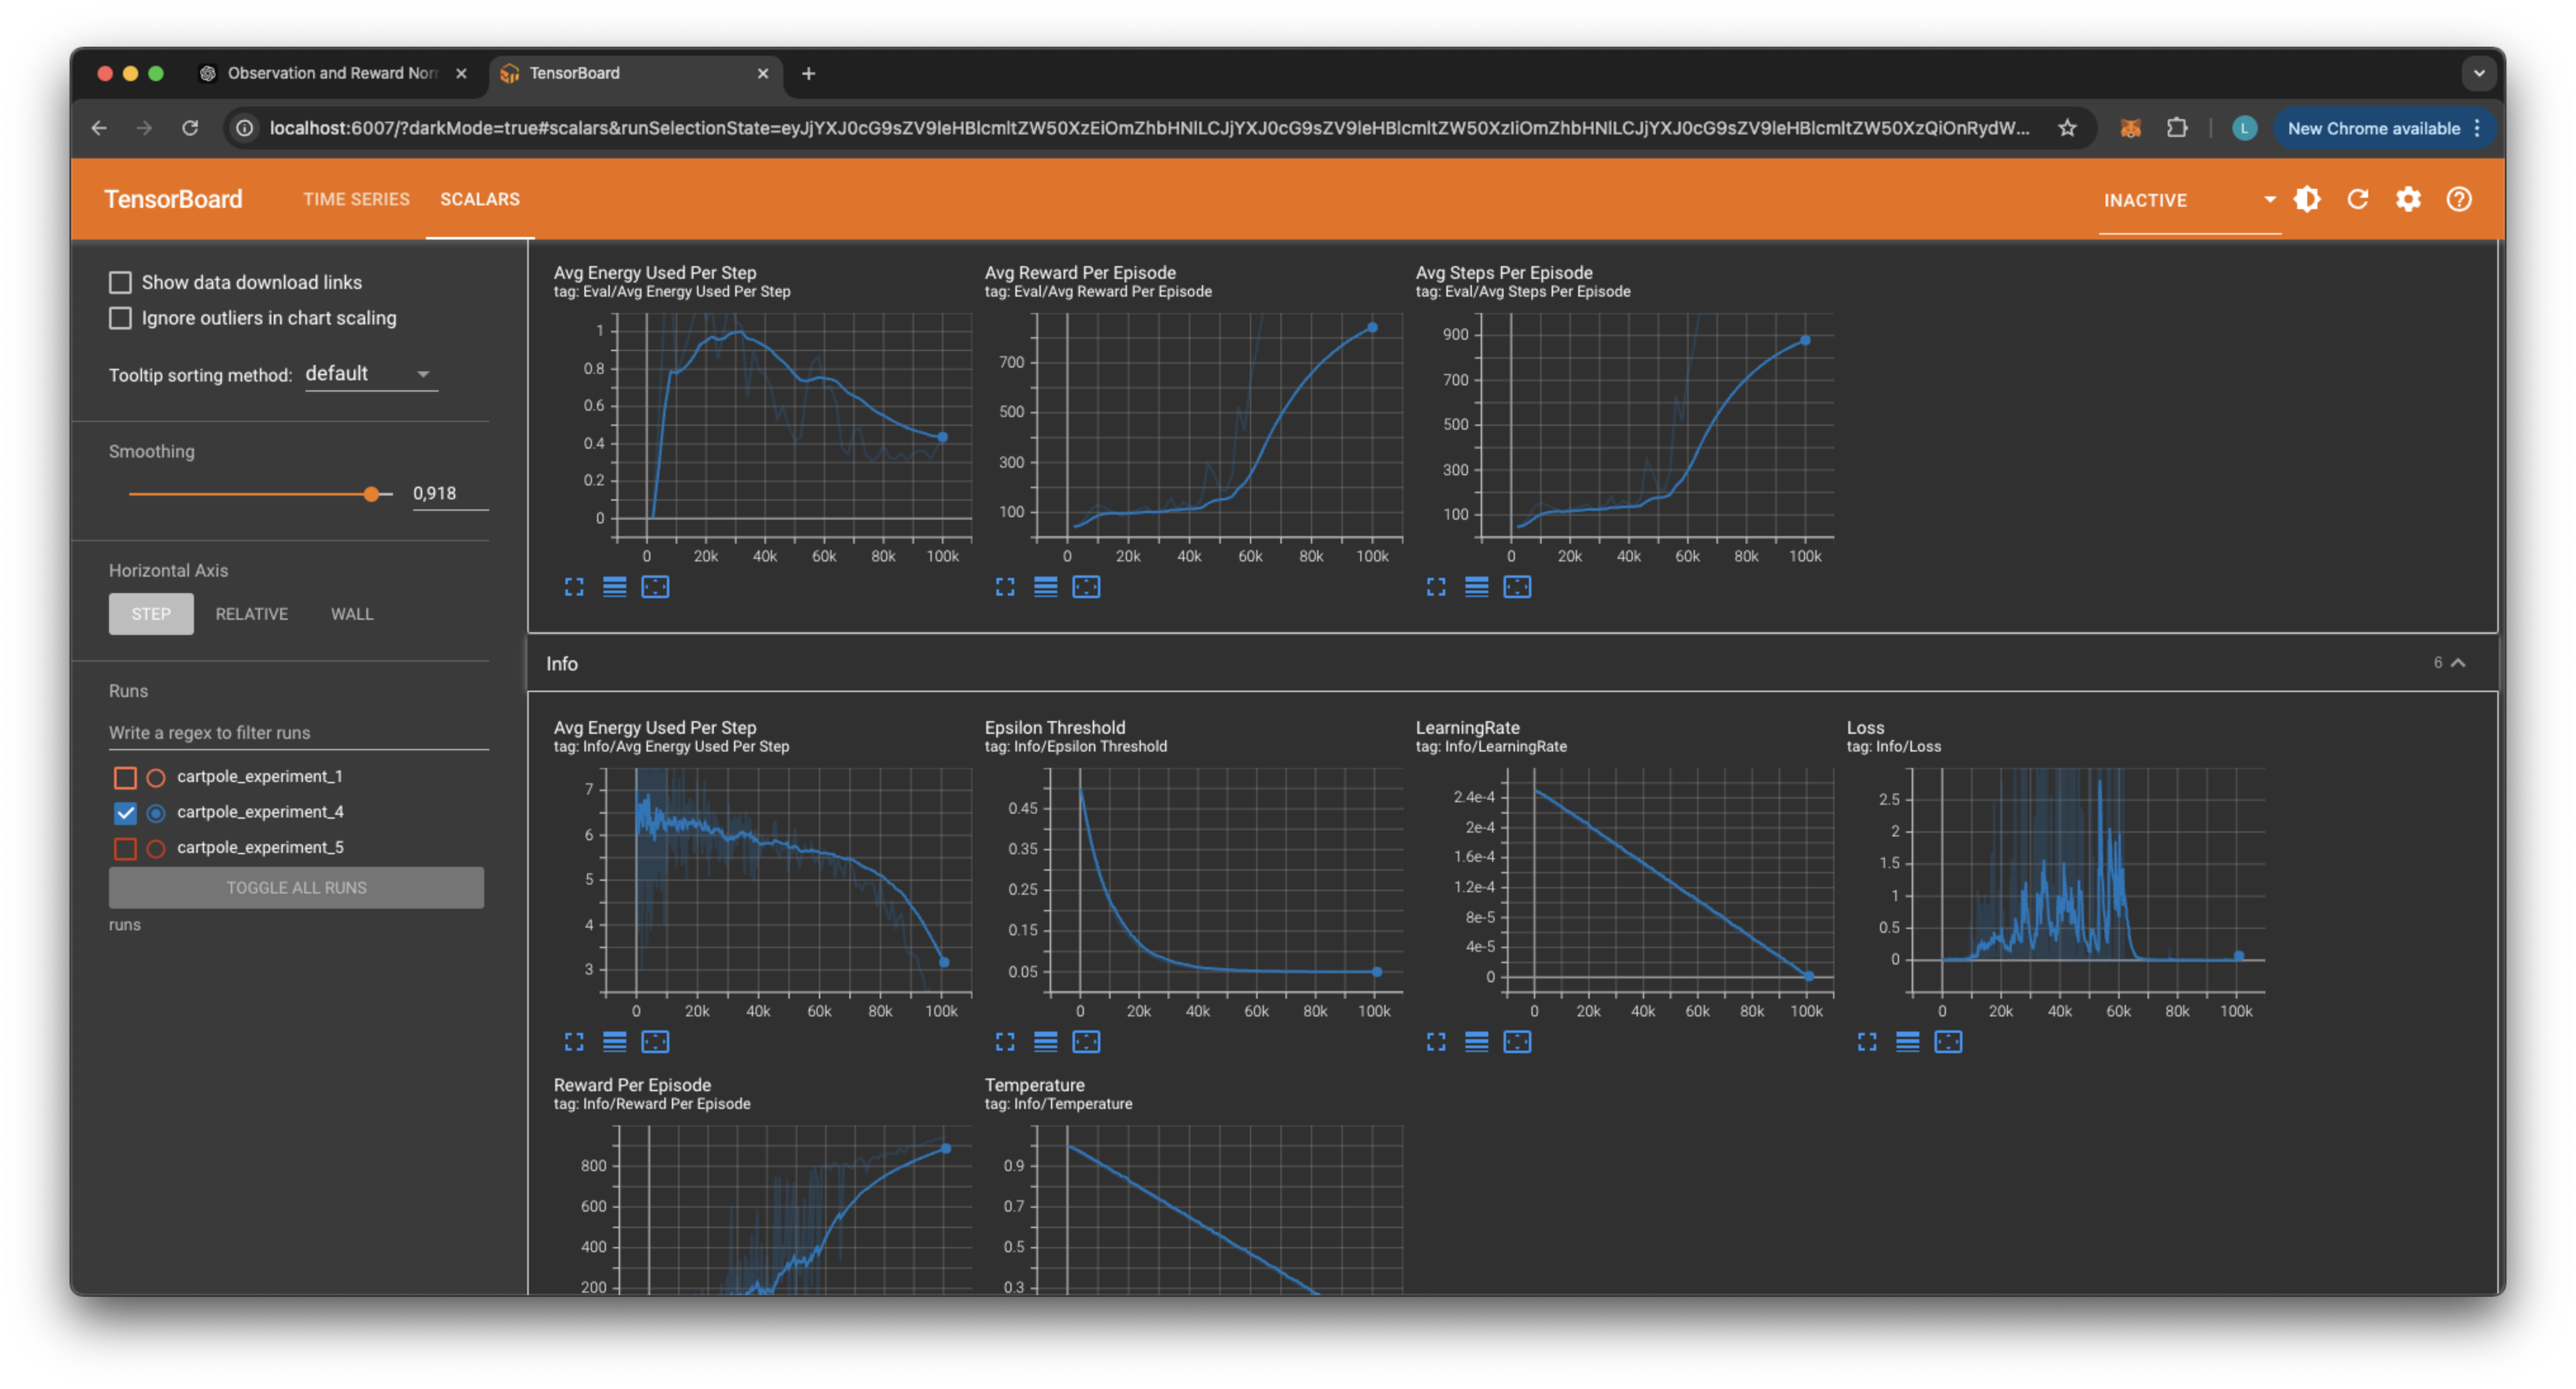
\includegraphics[width=1.0\textwidth]{images/tensorboard_dashboard.png}
    \caption{TensorBoard Dashboard showing training metrics}
    \label{fig:tensorboard_dashboard}
\end{figure}
\end{frame}

\begin{frame}
\frametitle{Algorithm Enhancements}
\begin{itemize}
    \item \textbf{Double DQN:} Mitigates overestimation bias by decoupling action selection and evaluation.
    \item \textbf{Prioritized Experience Replay:} Samples important transitions more frequently to accelerate learning.
    \item \textbf{Normalization:}
    \begin{itemize}
        \item \textit{Observation Normalization:} Stabilizes training by normalizing input features.
        \item \textit{Reward Normalization:} Ensures consistent reward scaling.
    \end{itemize}
    \item \textbf{Curriculum Learning:} 
    \begin{itemize}
        \item Phases:
        \begin{enumerate}
            \item \textbf{0-20k steps:} 50\% Alive Reward, 50\% Pole Angle Reward.
            \item \textbf{20k-50k steps:} 33\% Alive, 33\% Pole Angle, 33\% Distance to Center.
            \item \textbf{Above 50k steps:} 25\% each for Alive, Pole Angle, Distance to Center, and Energy Usage.
        \end{enumerate}
    \end{itemize}
\end{itemize}

\end{frame}


\begin{frame}
\frametitle{Algorithm Enhancements}
\begin{itemize}
    \item \textbf{Temperature-Scaled Softmax:}
    \begin{itemize}
        \item Initial Temperature: 1.0
        \item Final Temperature: 0.1
        \item Linearly decreases over training to reduce exploration over time.
    \end{itemize}
\end{itemize}

% TODO: Insert graphs showing loss stabilization with and without Prioritized Replay.
% Example Image: Loss curves comparing prioritized vs. uniform replay.
\begin{figure}[ht]
    \centering
    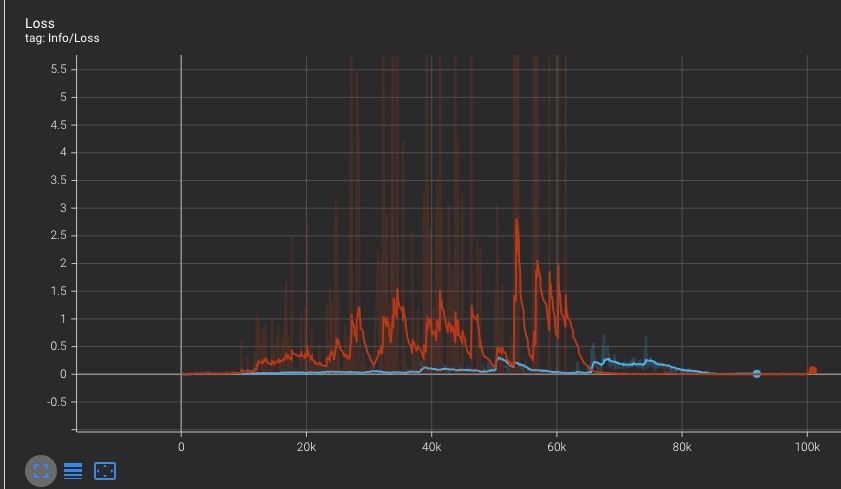
\includegraphics[width=0.7\textwidth]{images/loss_comparison.png}
    \caption{Loss Stabilization: Prioritized (blue) vs. Uniform Replay (red)}
    \label{fig:loss_comparison}
\end{figure}
\end{frame}

\section{Possible Extensions}

\begin{frame}
\frametitle{Possible Extensions}
\begin{itemize}
    \item \textbf{Stratification:} 
    \begin{itemize}
        \item Implement stratified sampling to ensure diverse experiences in replay buffer.
    \end{itemize}
    \item \textbf{Distribution-Aware Buffer:}
    \begin{itemize}
        \item Explore Cosine Similarity or Variational Autoencoders (VAEs) to model state distributions and enhance replay buffer sampling.
    \end{itemize}
    \item \textbf{Parallel Environments:}
    \begin{itemize}
        \item Increase to 16 parallel environments for faster experience collection and improved training efficiency.
    \end{itemize}
    \item \textbf{Reward Function Refinement:}
    \begin{itemize}
        \item Schedule Pole Angle and Distance to Center rewards to decrease over time, focusing more on energy optimization.
    \end{itemize}
    \item \textbf{Model Checkpointing:}
    \begin{itemize}
        \item Maintain multiple checkpoints to preserve best-performing models across different training phases.
    \end{itemize}
    \item \textbf{Advanced Exploration Strategies:}
    \begin{itemize}
        \item Incorporate other exploration methods like entropy regularization or intrinsic motivation (e.g., curiosity).
    \end{itemize}
\end{itemize}
\end{frame}

\section{Possible Shortcomings}

\begin{frame}
\frametitle{Possible Shortcomings}
\begin{itemize}
    \item \textbf{Algorithm Tuning:}
    \begin{itemize}
        \item Deep RL algorithms require extensive hyperparameter tuning for optimal performance.
    \end{itemize}
    \item \textbf{Overfitting:}
    \begin{itemize}
        \item The model may overfit to the specific environment configuration, limiting generalizability.
    \end{itemize}
    \item \textbf{Fixed Length Episodes:}
    \begin{itemize}
        \item Fixed-length episodes combined with energy consumption reward may lead to suboptimal behavior where the agent overfits to short-term gains.
    \end{itemize}
    \item \textbf{Training For Too Long Might Decrease Performance:}
    \begin{itemize}
        \item The agent might overfit to near-perfect behavior and forget more complex situations.
    \end{itemize}
    \item \textbf{Learning Stability:}
    \begin{itemize}
        \item Other on-policy algorithm like PPO might be more stable and efficient.
    \end{itemize}
\end{itemize}
\end{frame}

\section{Results and Analysis}

\begin{frame}
\frametitle{Results and Analysis}
\begin{itemize}
    \item \textbf{Training Outcome after 100k Steps:}
    \begin{itemize}
        \item \textbf{Average Reward:} 975/1000
        \item \textbf{Energy Consumption:} Under 0.4 per step (Full Power = 10 per step)
        \item \textbf{Success Rate:} 100\% during evaluation (No failures)
    \end{itemize}
    \item \textbf{Evaluation Strategy:}
    \begin{itemize}
        \item Conducted evaluations every 2k steps.
        \item Essential for monitoring performance due to off-policy learning, non-deterministic actions, and exploration.
    \end{itemize}
    \item \textbf{Prioritization Analysis:}
    \begin{itemize}
        \item Prioritized Experience Replay helped stabilize loss.
        \item Did not significantly enhance overall performance compared to uniform sampling.
    \end{itemize}
\end{itemize}

% TODO: Insert TensorBoard screenshots showing reward progression and energy consumption.
% Example Image: TensorBoard graphs for Reward, Energy Consumption, and Success Rate over training steps.
\begin{figure}[ht]
    \centering
    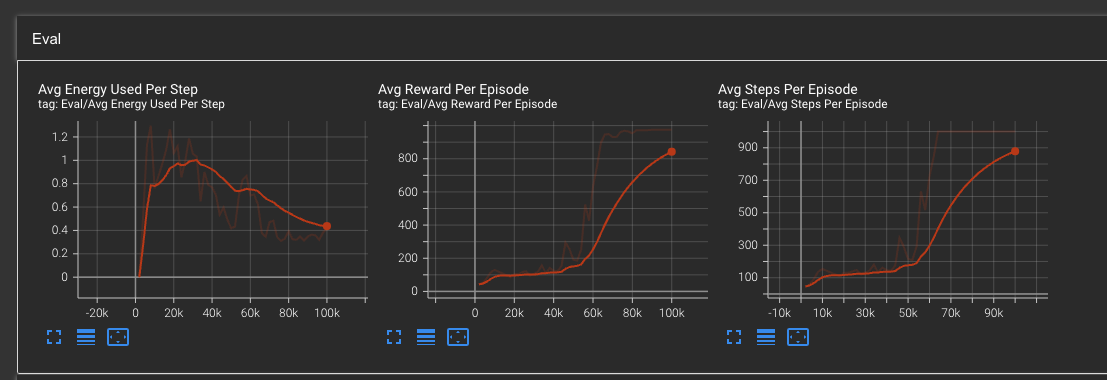
\includegraphics[width=0.7\textwidth]{images/tensorboard_metrics.png}
    \caption{Training Metrics: Reward, Energy Consumption, and Success Rate}
    \label{fig:tensorboard_metrics}
\end{figure}
\end{frame}

\section{Conclusion}

\begin{frame}
\frametitle{Conclusion}
\begin{itemize}
    \item Successfully enhanced the CartPole environment with a third "Do Nothing" action and optimized reward structure for energy consumption.
    \item Developed a robust deep RL solution incorporating curriculum learning and temperature-scaled softmax for effective exploration-exploitation balance.
    \item Achieved high performance with minimal energy usage and a perfect success rate in evaluations.
    \item Identified areas for improvement, including further algorithm tuning and exploring advanced buffer management techniques.
\end{itemize}
\end{frame}

\end{document}
